% \documentclass{article}
% \usepackage[utf8]{inputenc}
% \usepackage{amsmath}
% \usepackage{graphicx}
% \usepackage{listings}
% \usepackage[top=1.55cm, bottom=2.29cm, left=1.6cm, right=1.47cm]{geometry}
% This is for the fancy title in each page
%\rhead{Software Requirements Specification}
%\lhead{}
%\chead{}
%\rhead{In-hand object detection and tracking using 2D and 3D information}
% \pagestyle{empty}

% \usepackage{enumitem}


% \makeatletter
% \def\threedigits#1{\expandafter\@threedigits\csname c@#1\endcsname}
% \def\@threedigits#1{%
%   \ifnum#1<100 0\fi
%   \ifnum#1<10 0\fi
%   \number#1}
% \makeatother
% \AddEnumerateCounter{\threedigits}{\@threedigits}{100}
% \usepackage{hyperref}
% \hypersetup{
%     pdfauthor={Irene Sanz Nieto},
%     colorlinks,
%     citecolor=blue,
%     filecolor=blue,
%     linkcolor=blue,
%     urlcolor=blue,
% }

% \usepackage{float}

%\setenumerate[1]{}


% \begin{document}

% %%%% FRONTPAGE %%%%%%%%%%%%%%%%%%%%%%%%%%%%%%%%%%%%%%%%%%%%%%%%%%%%%%%%%%%
% \begin{titlepage}

% \begin{center}
% %
\includegraphics[width=0.25\textwidth]{./uc3m.jpg}\\[2cm]
% \textsc{\huge Bachelor's Thesis:\\[0.5cm]In-hand object detection and tracking using\\[0.5cm]2D and 3D
% information }\\[4cm]


% % Title
% {\Huge\bfseries{Software Requirements Specification}\\[2cm]}

% \Large{Version 1.0}
% \\[11cm]


% % Author and supervisor
% \begin{minipage}{0.55\textwidth}
% \begin{flushleft} \large
% \emph{Author:}\\
% Irene Sanz Nieto\\
% \end{flushleft}
% \end{minipage}
% \begin{minipage}{0.4\textwidth}
% \begin{flushright} \large
% \emph{Supervisor:}\\
% Victor González Pacheco\end{flushright}\end{minipage}\vfill

% % Bottom of the page
% %{\large \today}

% \end{center}
% \end{titlepage}

%
\newpage
%
%%%%%%Table of contents%%%%%%%%%%%%%%%%%%%%%%%%%%%%%%
%%%%%%%%%%%%%%%%%%%%%%%%%%%%%%%%%%%%%%%%%%%%%%%%%%%%%
\tableofcontents
%%%%%% TABLE OF FIGURES %%%%%%
\listoffigures

\newpage


%%%%%%Document%%%%%%%%%%%%%%%%%%%%%%%%%%%%%%%%%%
%%%%%%%%%%%%%%%%%%%%%%%%%%%%%%%%%%%%%%%%%%%%%%%%%%%%%
\section{Introduction}
\hspace{0.5cm}The project consists on an in-hand object learning and recognition software. 
The project is conceived for being used in a robot. In a robot there are numerous processes that have to run in parallel to avoid a lose of information and be able to work and respond in real time. 
\\
To fulfill this request, the code has been subdivided in nodes that perfom simple tasks and that are executed simultaneously. 
\\
The nodes that appear in the project are the following : 

%include the new picture!!
\begin{itemize}
\item Converter : \\
There exists a converter node that transforms the pi\_ tracker message into the custom message HandLoc. This transformation is made extracting only the information regarding the hands and their name and copying it into the correct fields of the new message. 
This message is the one being used in the rest of the project's code. Hence, this node is the one that connects the thesis ROS package with the pi\_ tracker package.

\item ROI Segmenters:\\ 
These nodes work using the previous node's information. They extract the Region Of Interest (ROI) from the raw input information. Since the information that the project can analyze is both in 2D and 3D, there will be two ROI Segmenters, one for each type of information. 
Those two ROI Segmenter nodes run in parallel but they depend in each other. The actual segmentation is made with the 3D data. The result is two new point clouds with the hands.
After the 3D segmentation, the maximum and minimum coordinates of each of the hands' point clouds are transformed to pixels in order to segment the 2D ROI. 

\item Feature Extractors: \\
As the ROI Segmenters, there will be two nodes to extract the features. One extracts the 3D features from the segmented point cloud and the other one extracts the 2D features from the segmented picture. 
The features are characteristics of interest of the objects whose value can be used to discriminate between objects and hence distinguish some objects within a set of different data. 


\item Learner: \\
This node implements the learning sequence of new objects and also the training of the algorithm specified in the functional requirements section. 
It uses the features (both 2D and 3D) extracted from the previous node to make the training. 

\item Recogniser:\\ 
This node implements the recognizing sequence. It compares the features extracted at each captured frame using the previously trained algorithms. 
\end{itemize}
   
The communication between nodes is made using the Robotic Operating System topics. The nodes can publish in a specific topic a certain message or subscribe to that topic to retrieve the message. 
There are different types of messages depending on the information that has to be transmitted. There exist certain ROS libraries that define standard messages or geometric messages as an example. It is also possible to create a custom message type. 


\subsection{Nodes}

\subsubsection{Converter Node}

This node converts the messages from other ROS packages to the internal message format used within the code. 
Figure \ref{uc_converter} presents the use case diagram of the node. 

\begin{figure}[H]
\begin{center}
	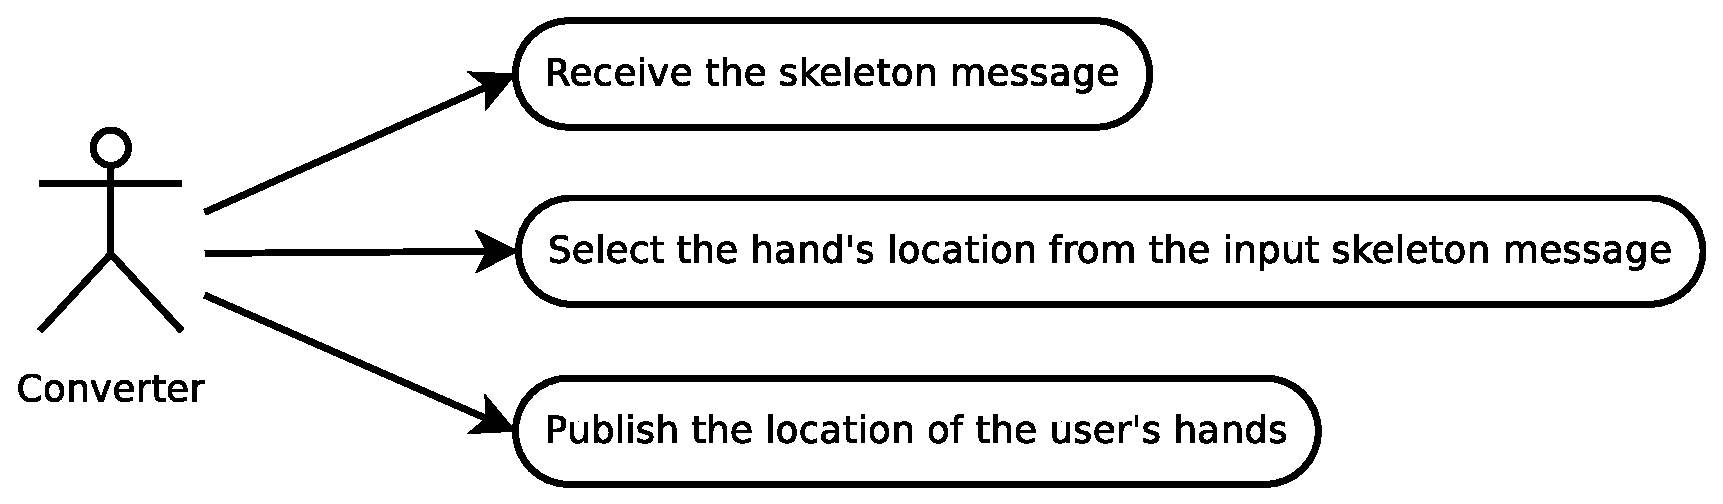
\includegraphics[scale=0.4]{img/diagrams/uc_converter.eps}
			\caption[Use case diagram converter node]{Use Case diagram of the converter node}
		\label{uc_converter}
\end{center}
\end{figure}
	
\subsubsection{ROI Segmenter Nodes}
There are two nodes that extract the ROI (Region Of Interest), one for the 2D and the other one for the 3D data.

\paragraph {ROI Segmenter 3D Node\\[0.5cm]}

The first region of interest segmented is the 3D. Using the hand's center position obtained from the pi\_ tracker ROS package a prism is extracted around it. Its dimensions are all fixed to an experimental value that is suitable for this purpose. 
No outlier filtering is done due to the high computing time required.  
The limits of the 3D ROI extracted are converted to pixels and published in a topic. These limits are the inputs of the following node. 
Figure \ref{uc_roi3d} shows the use case diagram of the node. 

\begin{figure}[H]
\begin{center}
	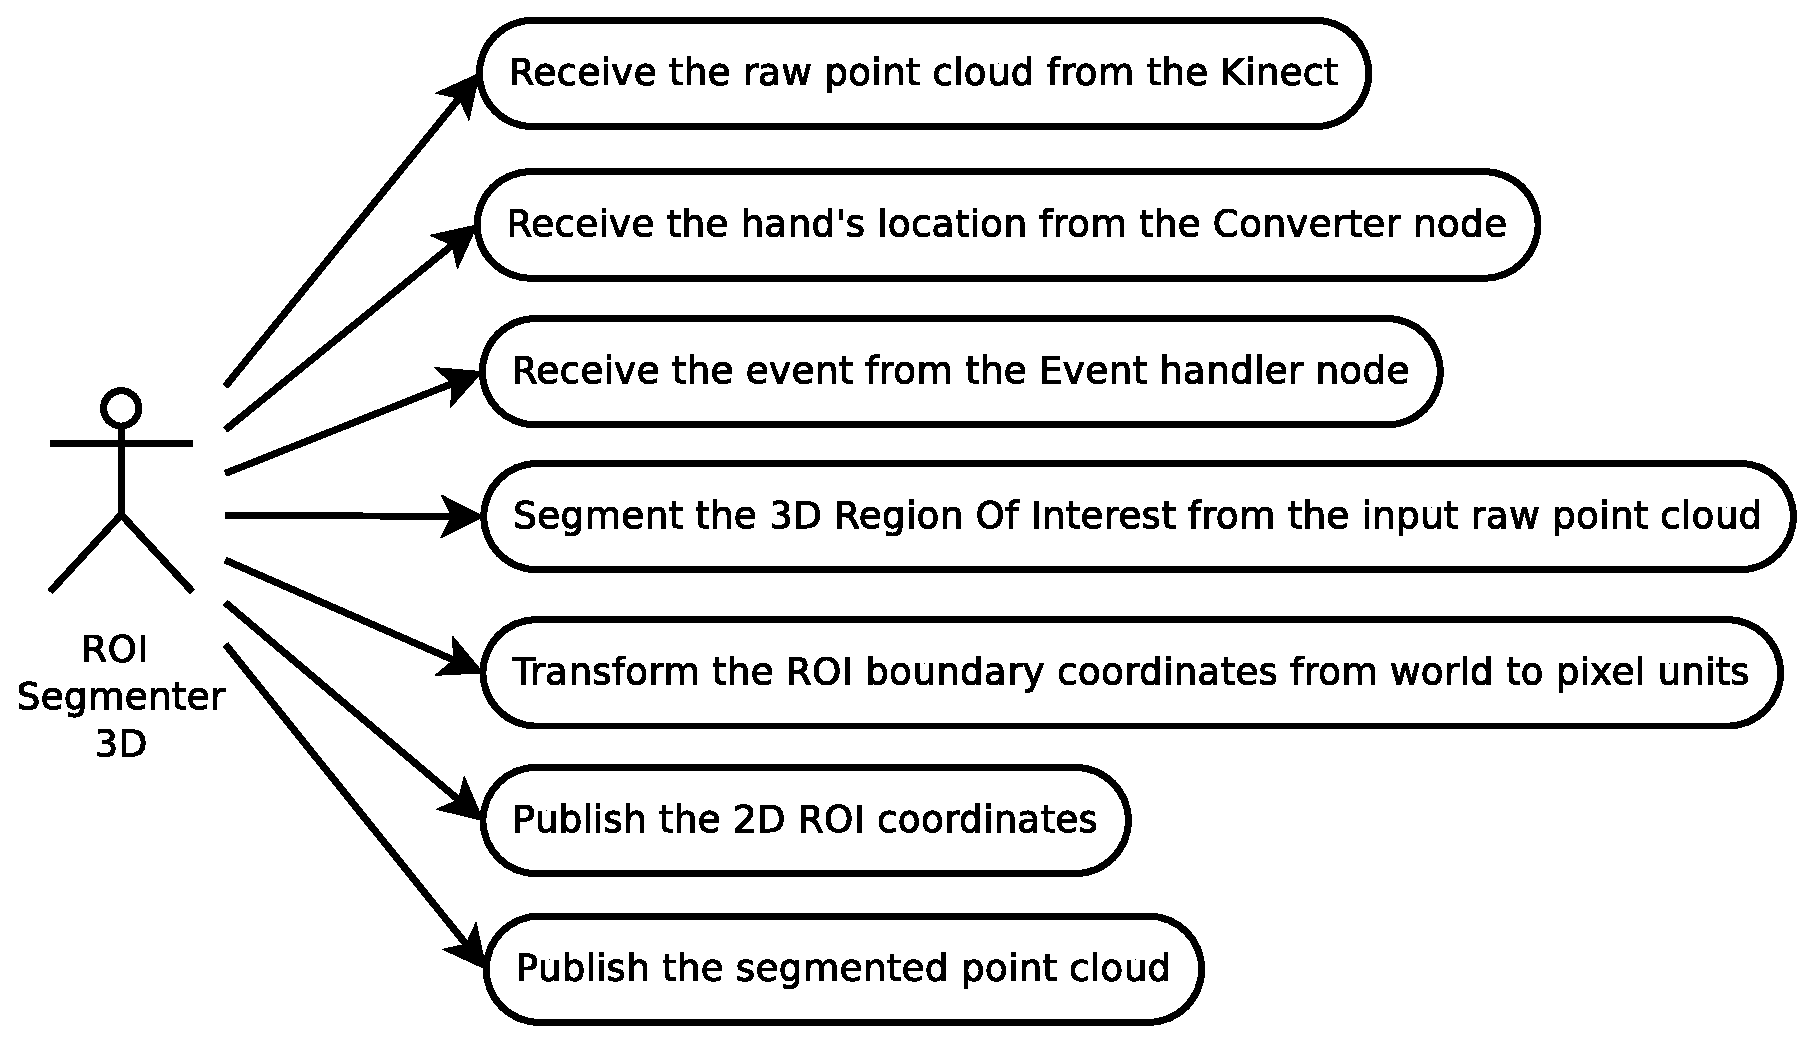
\includegraphics[scale=0.4]{img/diagrams/uc_roi_segmenter_3d.eps}
			\caption[Use case diagram ROI segmenter 3D node]{Use Case diagram of the ROI segmenter 3D node}
		\label{uc_roi3d}	

\end{center}
\end{figure}

\paragraph{ROI Segmenter 2D Node\\[0.5cm]}
As it was previously mentioned, the 2D ROI dimensions are extracted from the 3D ROI. The original image obtained from the RGB-D sensor is cropped using those points. 
The outputs of this node are two topics, one with the 2D ROI (a custom message that includes an image and a name) and the other one with the 3D ROI (a point cloud).
To decrease the computation time, the point clouds do not have the RGB component. Thus, the color information is obtained through the 2D ROI. 
Figure \ref{uc_roi2d} presents the use case of this node. 
\begin{figure}[H]
\begin{center}
	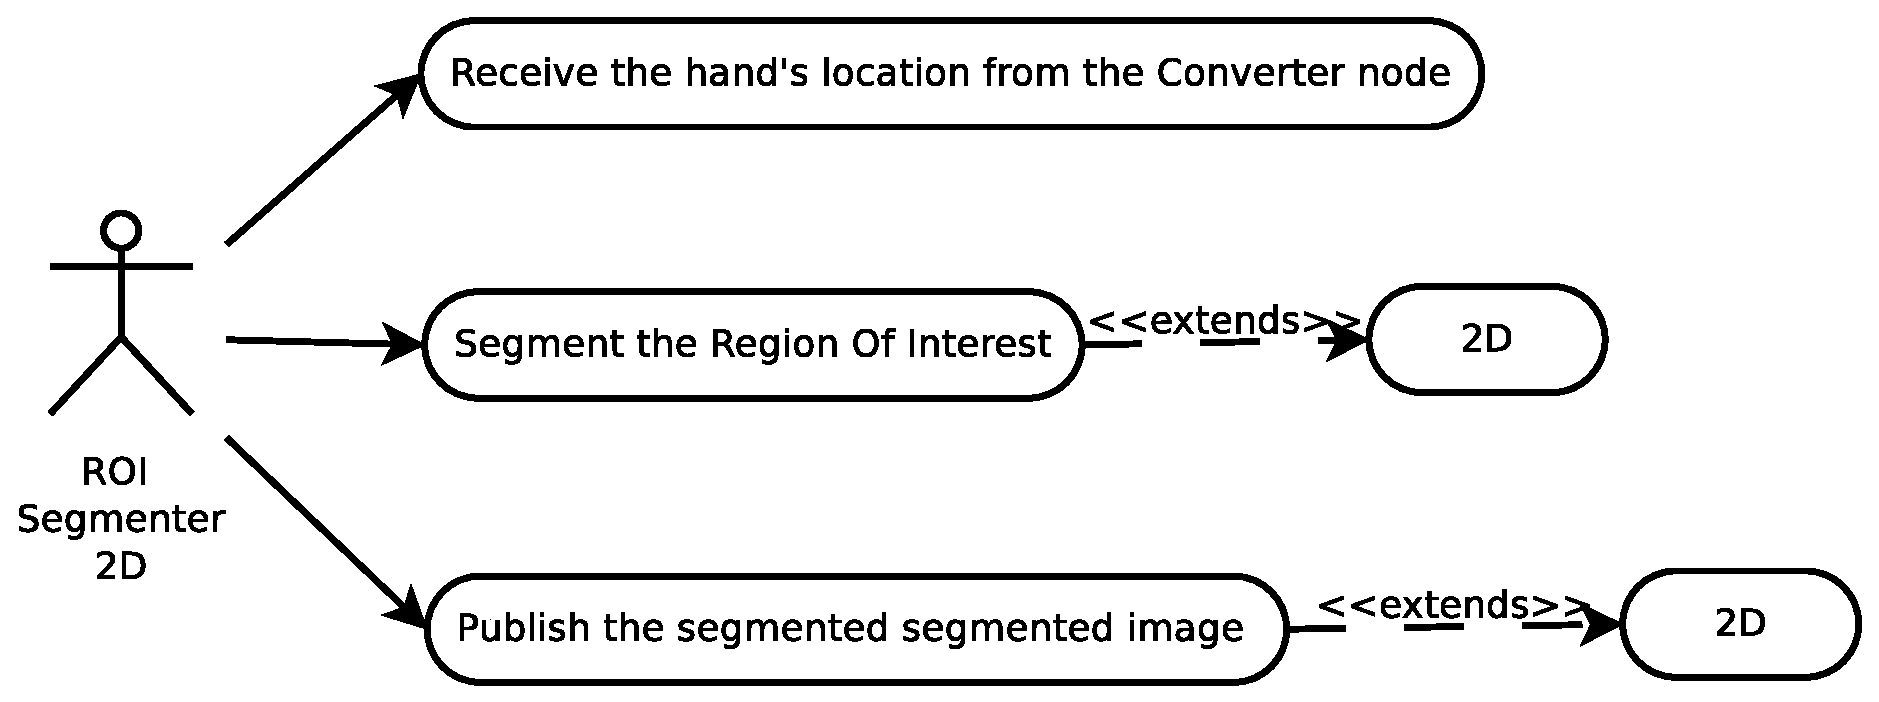
\includegraphics[scale=0.4]{img/diagrams/uc_roi_segmenter_2d.eps}
			\caption[Use case diagram ROI segmenter 2D node]{Use Case diagram of the ROI segmenter 2D node}
		\label{uc_roi2d}
\end{center}
\end{figure}

\subsubsection{Feature Extractor Nodes}
\paragraph{Feature Extractor 2D Node \\[0.5cm]}
This node is used to extract the descriptors or features from the 2D Region Of Interest. 
The use case diagram may be found in figure \ref{uc_fe2d}
\begin{figure}[H]
\begin{center}
	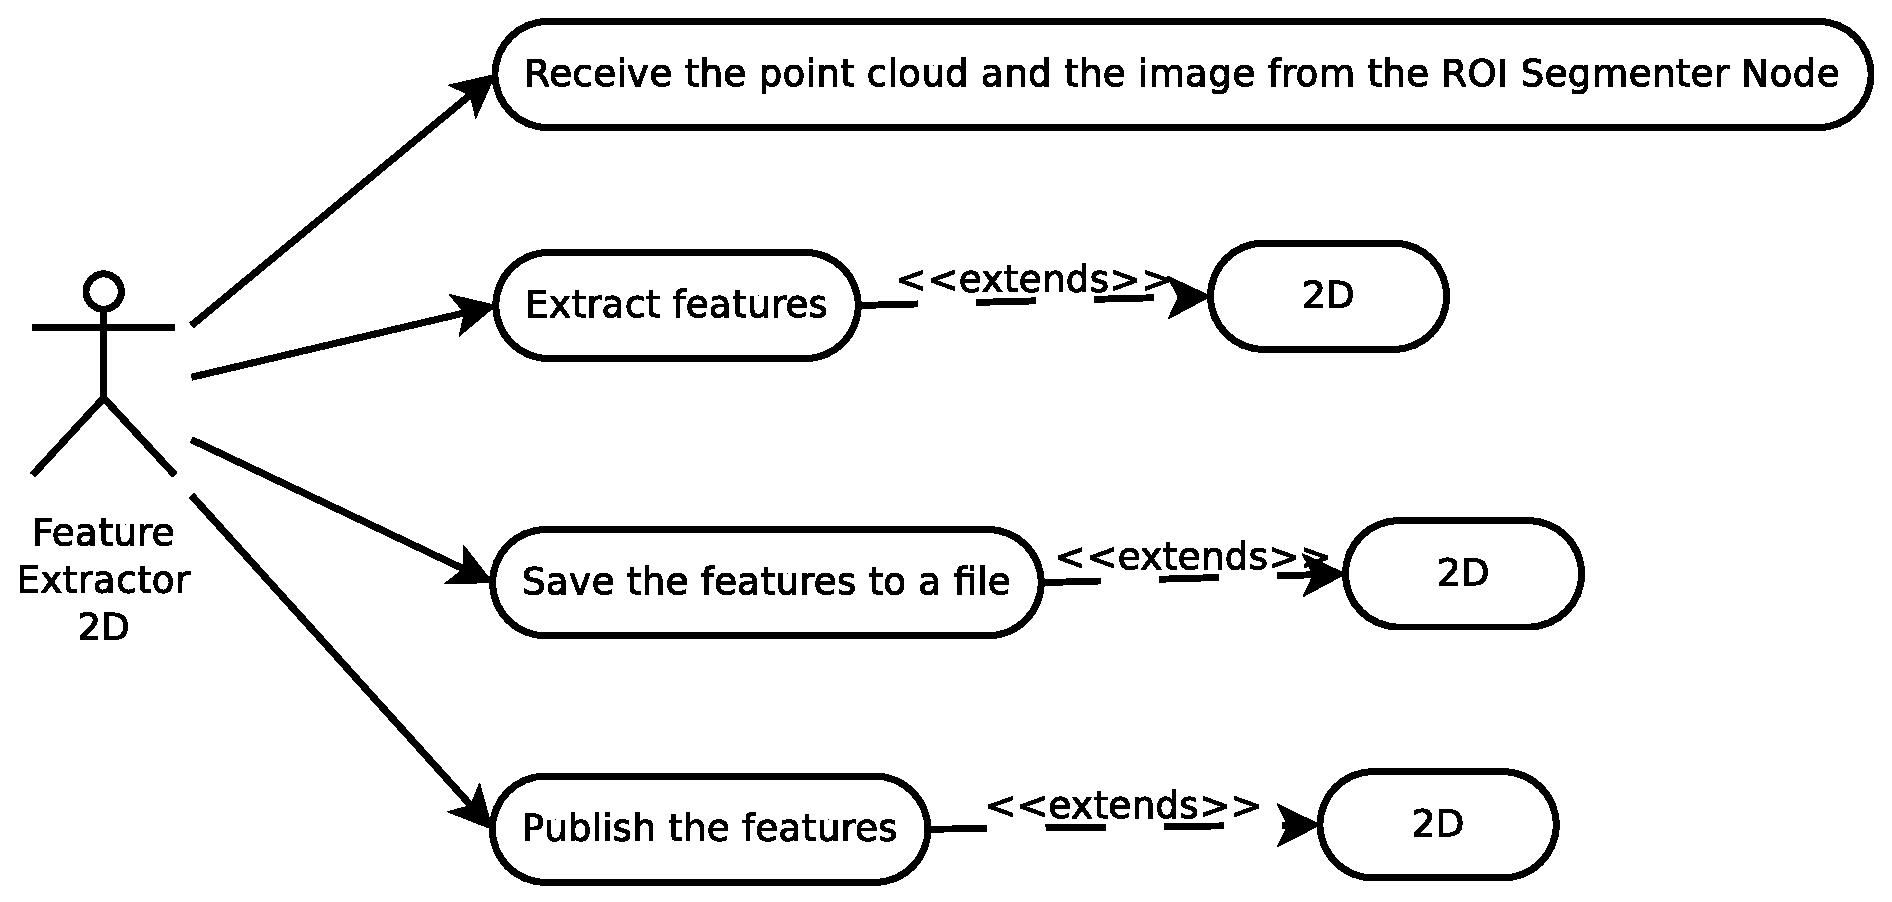
\includegraphics[scale=0.4]{img/diagrams/uc_feature_extractor_2d.eps}
			\caption[Use case diagram Feature Extractor 2D node]{Use Case diagram of the Feature Extractor 2D node}
		\label{uc_fe2d}
\end{center}
\end{figure}


\paragraph{Feature Extractor 3D Node \\[0.5cm]}
Similarly to the feature extractor 2D node, this node extracts the descriptors from the 3D ROI. 
Its use case diagram is shown in figure \ref{uc_fe3d}.
\begin{figure}[H]
\begin{center}
	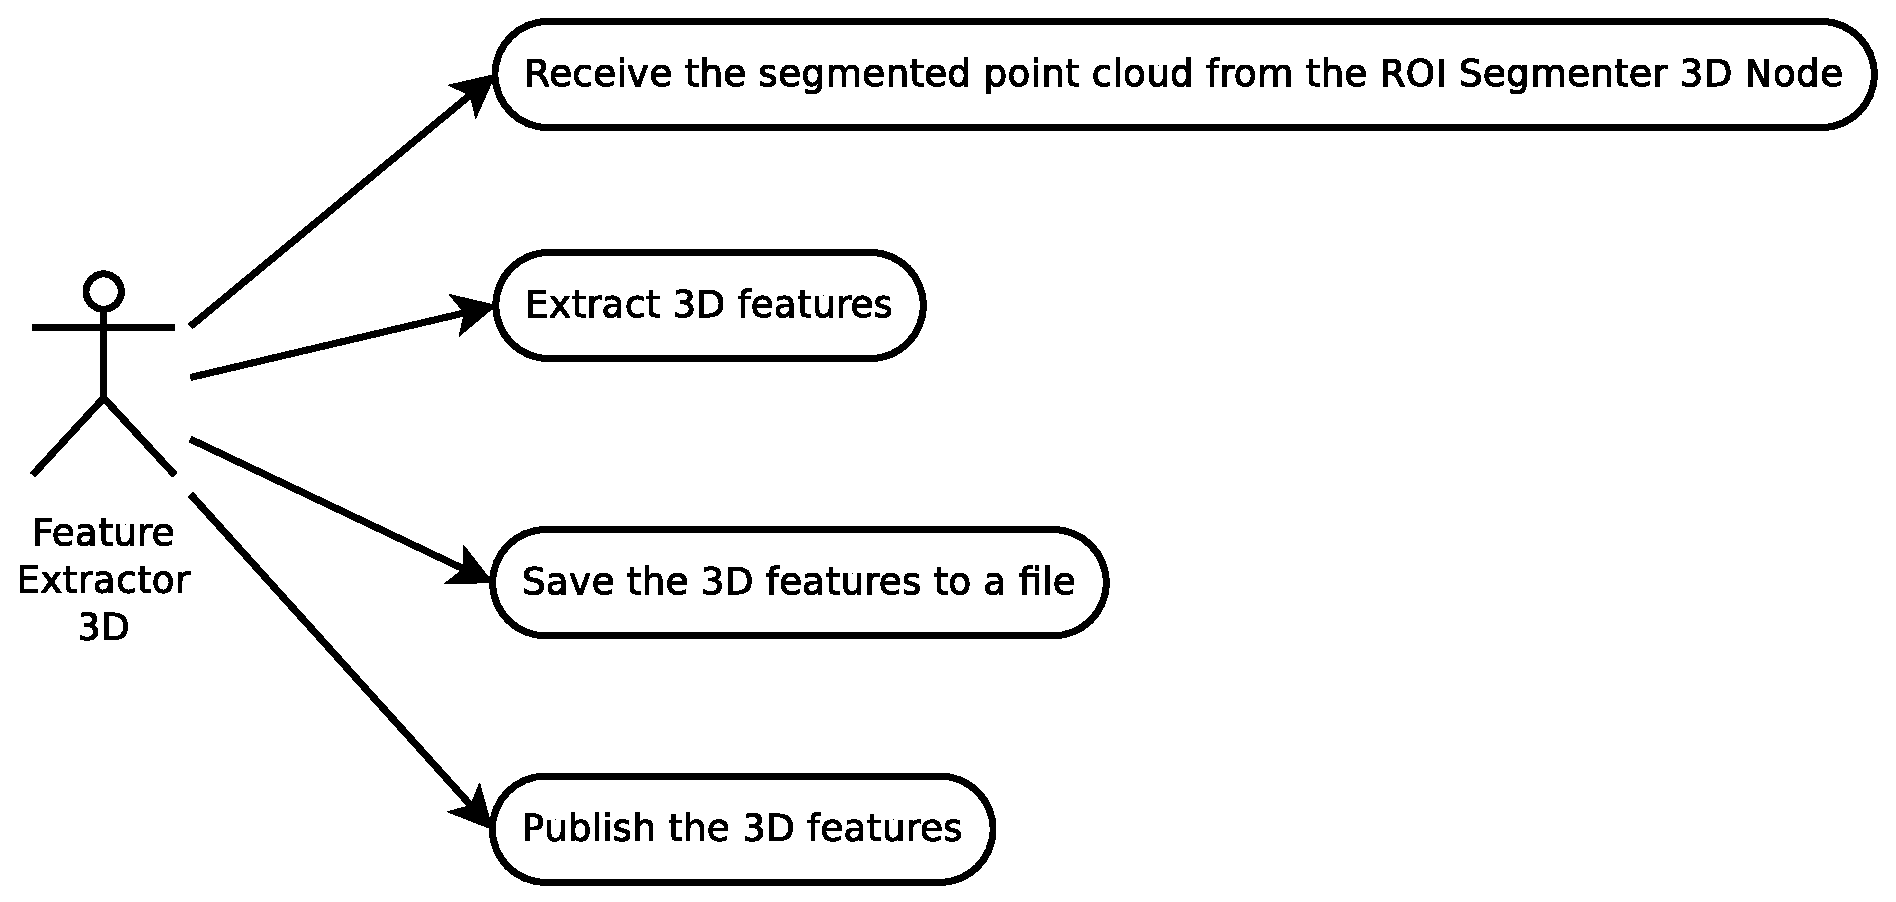
\includegraphics[scale=0.4]{img/diagrams/uc_feature_extractor_3d.eps}
			\caption[Use case diagram Feature Extractor 3D node]{Use Case diagram of the Feature Extractor 3D node}
		\label{uc_fe3d}
\end{center}
\end{figure}


% \subsubsection{Data Parser Node}
% This node stores the 2D and 3D features of each template of the same object in one file. 
% \begin{figure}[H]
% \begin{center}
% 	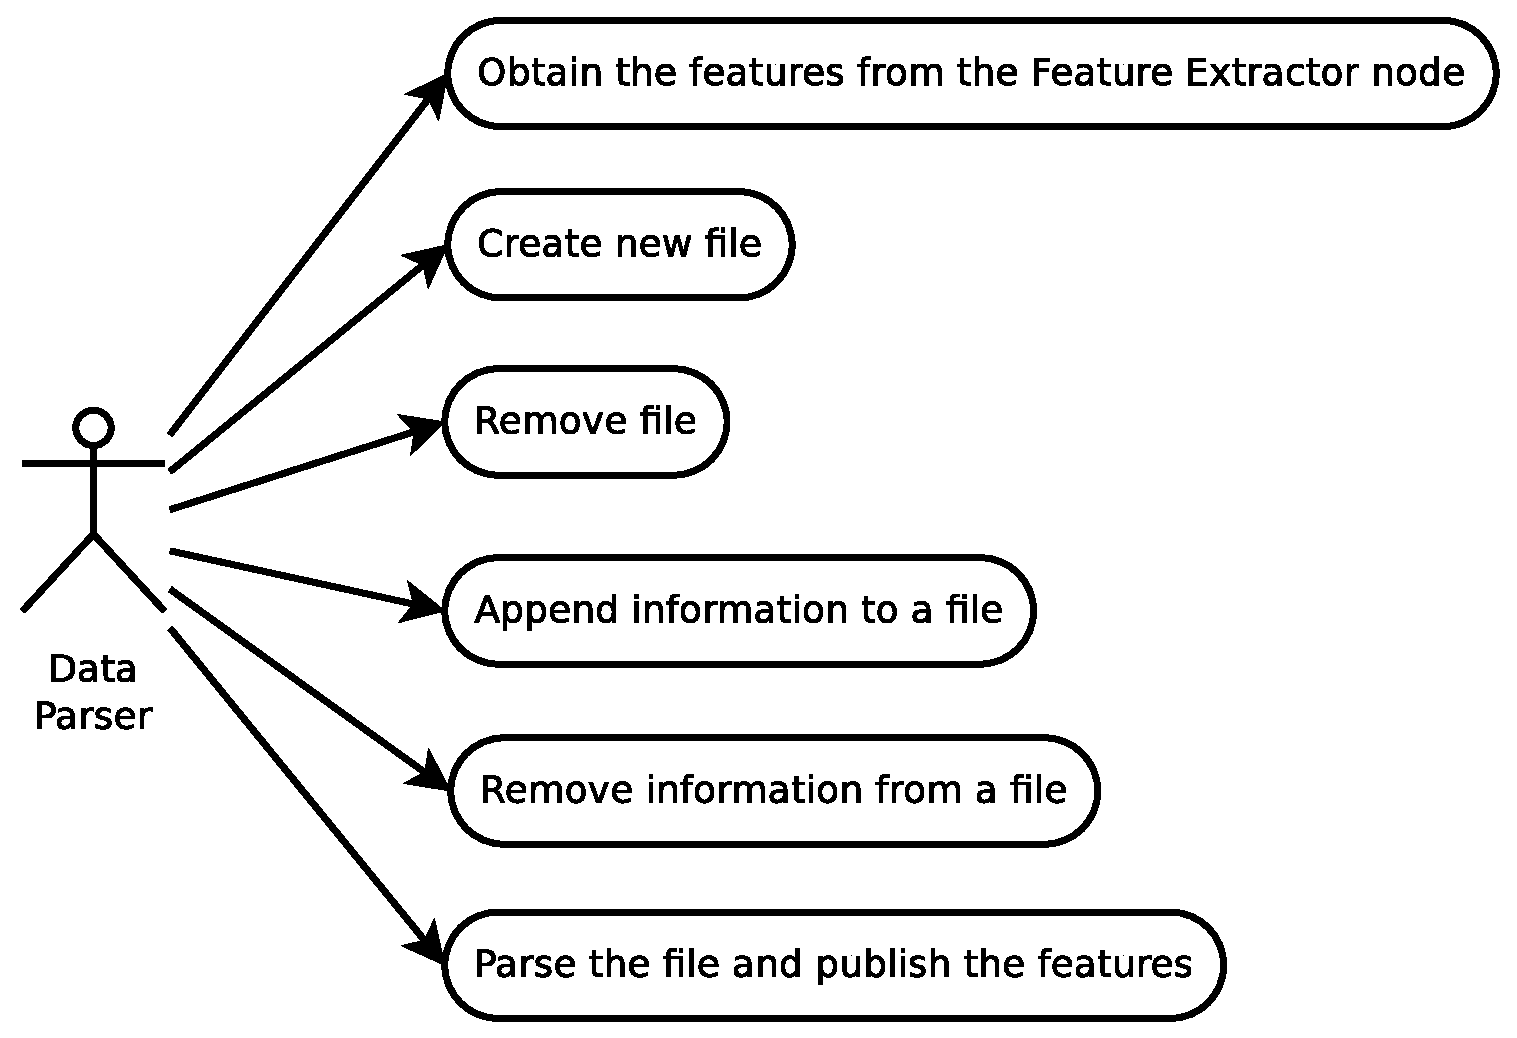
\includegraphics[scale=0.4]{img/diagrams/uc_data_parser.eps}
% \end{center}
% \end{figure}


\subsubsection{Event Handler Node}
	This node identifies the different user's gestures and publishes the current event.
	Its use case diagram may be found in figure \ref{uc_event}. 

	\begin{figure}[H]
\begin{center}
		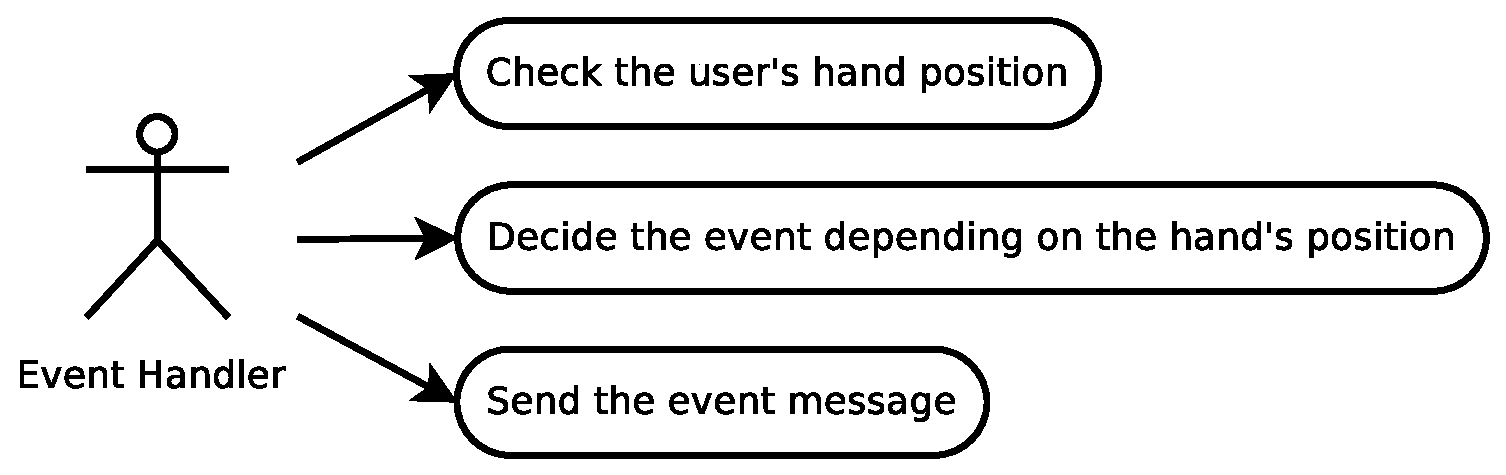
\includegraphics[scale=0.4]{img/diagrams/uc_event_handler.eps}

	\end{center}
	\caption[Use case diagram Event Handler node]{Use Case diagram of the Event Handler node}
		\label{uc_event}
\end{figure}
	
	
\subsubsection{Learner Recognizer Node}

\hspace{0.5cm}This node implements the state machine algorithm. It has two differentiated modes: learning and recognizing. 

\begin{itemize}

\item{Learning\\}

This mode learns 2D and 3D features extracted from the handheld object using a RGB-D sensor.   
The sequence of the object learning is the following:
\\
First, 3D and 2D descriptors are extracted and written to a file. Then, two algorithms are trained (one for 2D and the other for the 3D template). The parameters of each trained algorithm are stored in a file. There will be hence one file per learned object and one file per algorithm.
\\

The learning of the objects is done in-hand. The training starts when the user extends the hand in front of the body, showing the new object to the RGB-D sensor. Then, the user rotates the object to allow the software to extract the features of different views to obtain a more robust model of the object. This way of learning new objects will allow a more intuitive interaction human-robot. When the user returns the arm to a position which is closer to the body, the algorithm starts learning the new object and after the learning, it comes back to the recognizing mode, which is the default. 


\item{Recognizing\\}

This mode tracks the user's hands and recognizes the held objects. 

There are two different algorithms, one trained with the 2D data and the other one trained with the 3D data. More information about those algorithms may be found in the Functional Requirements section. 
\\
The steps done by this mode are the following: 
First, as in the Learning Mode, 2D and 3D descriptors are extracted. Then, the algorithms will compare that information with the learned one. 
The output of each algorithm will be a percentage of similarity between the dataset and the new object. 
The 3D information is more reliable than the 2D. The latter is subjected to inaccuracies due to illumination or view angle that affects the descriptors extracted and hence the object recognition.
Due to this fact, weights for the output of each algorithm will be given. Those give a higher importance to the 3D descriptors since they are more robust. 
\\
The object that is finally published in a topic will be the one with a higher percentage of similarity. 



\begin{figure}[H]
\begin{center}

		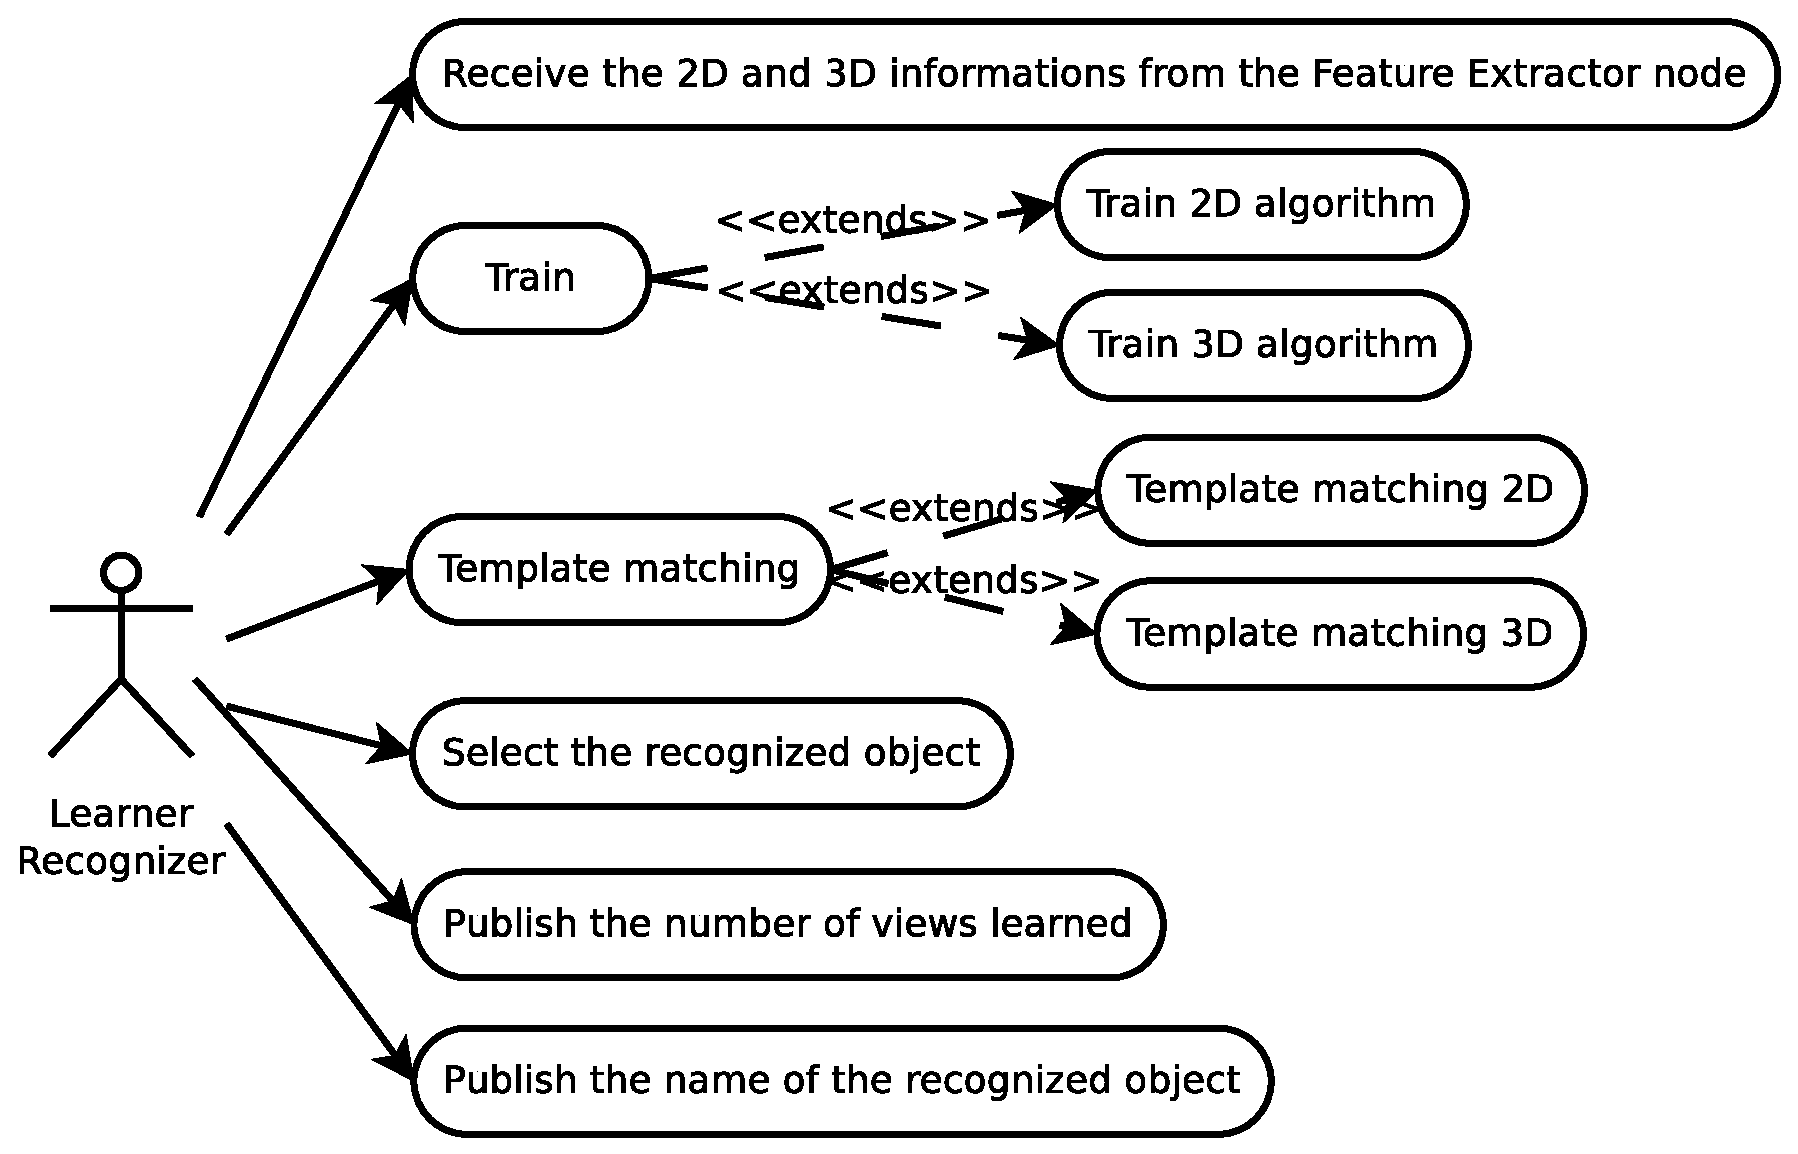
\includegraphics[scale=0.4]{img/diagrams/uc_learner_recognizer.eps}
	\end{center}
\end{figure}



\end{itemize}

% \subsubsection{Object Recognizer Node} 


% \begin{figure}[H]
% \begin{center}
% 	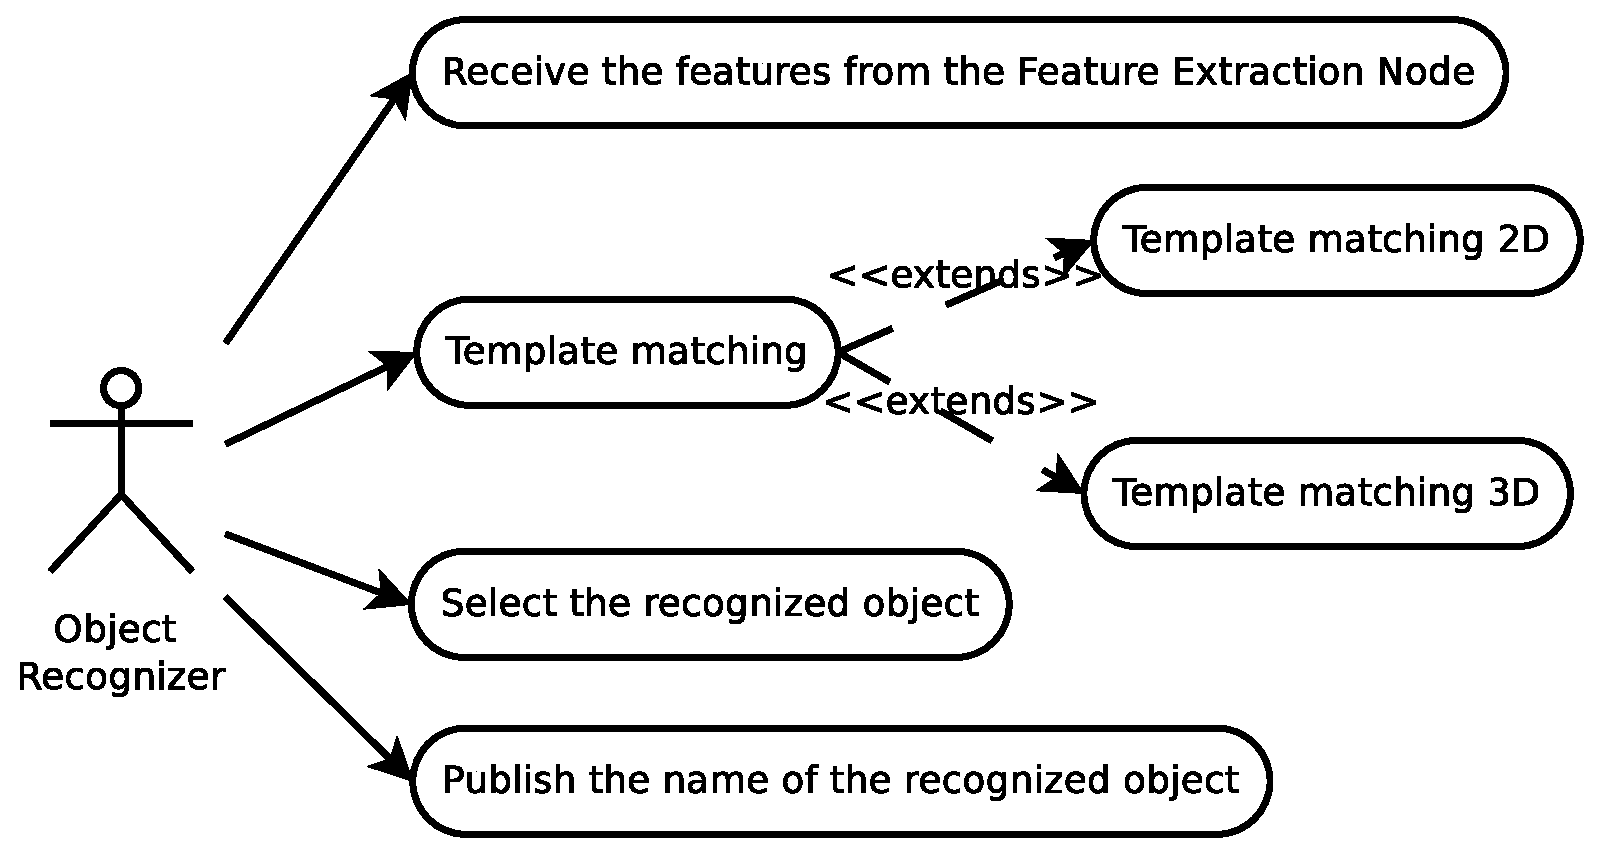
\includegraphics[scale=0.4]{img/diagrams/uc_recognizer.eps}
% \end{center}
% \end{figure}


\subsection{Third Party Packages}
\hspace{0.5cm}In this project, three third party libraries are being used: pi\_ tracker, OpenCV, PCL. 
\subsubsection{ Pi\_ tracker}
Pi\_ tracker is a ROS package that publishes the position and orientation of each joint of the users. From that information, the location of both hands of the user is extracted and used in the rest of the software. 
\subsubsection{ OpenCV}
This real-time computer vision library is used mainly to extract and compare the features of the objects in 2D. 
\subsubsection{PCL}
This open-source framework implements different algorithms for n-dimensional point clouds and 3D geometry processing.
In this project, it is used to filter, extract features and segment the RGB-D's point clouds.

\subsection{Node Interaction}
In the following diagram it can be seen the interaction and the information exchanged between nodes.
%\subsubsection{Use Case Diagram}
%\begin{figure}[H]
% \begin{center}
% %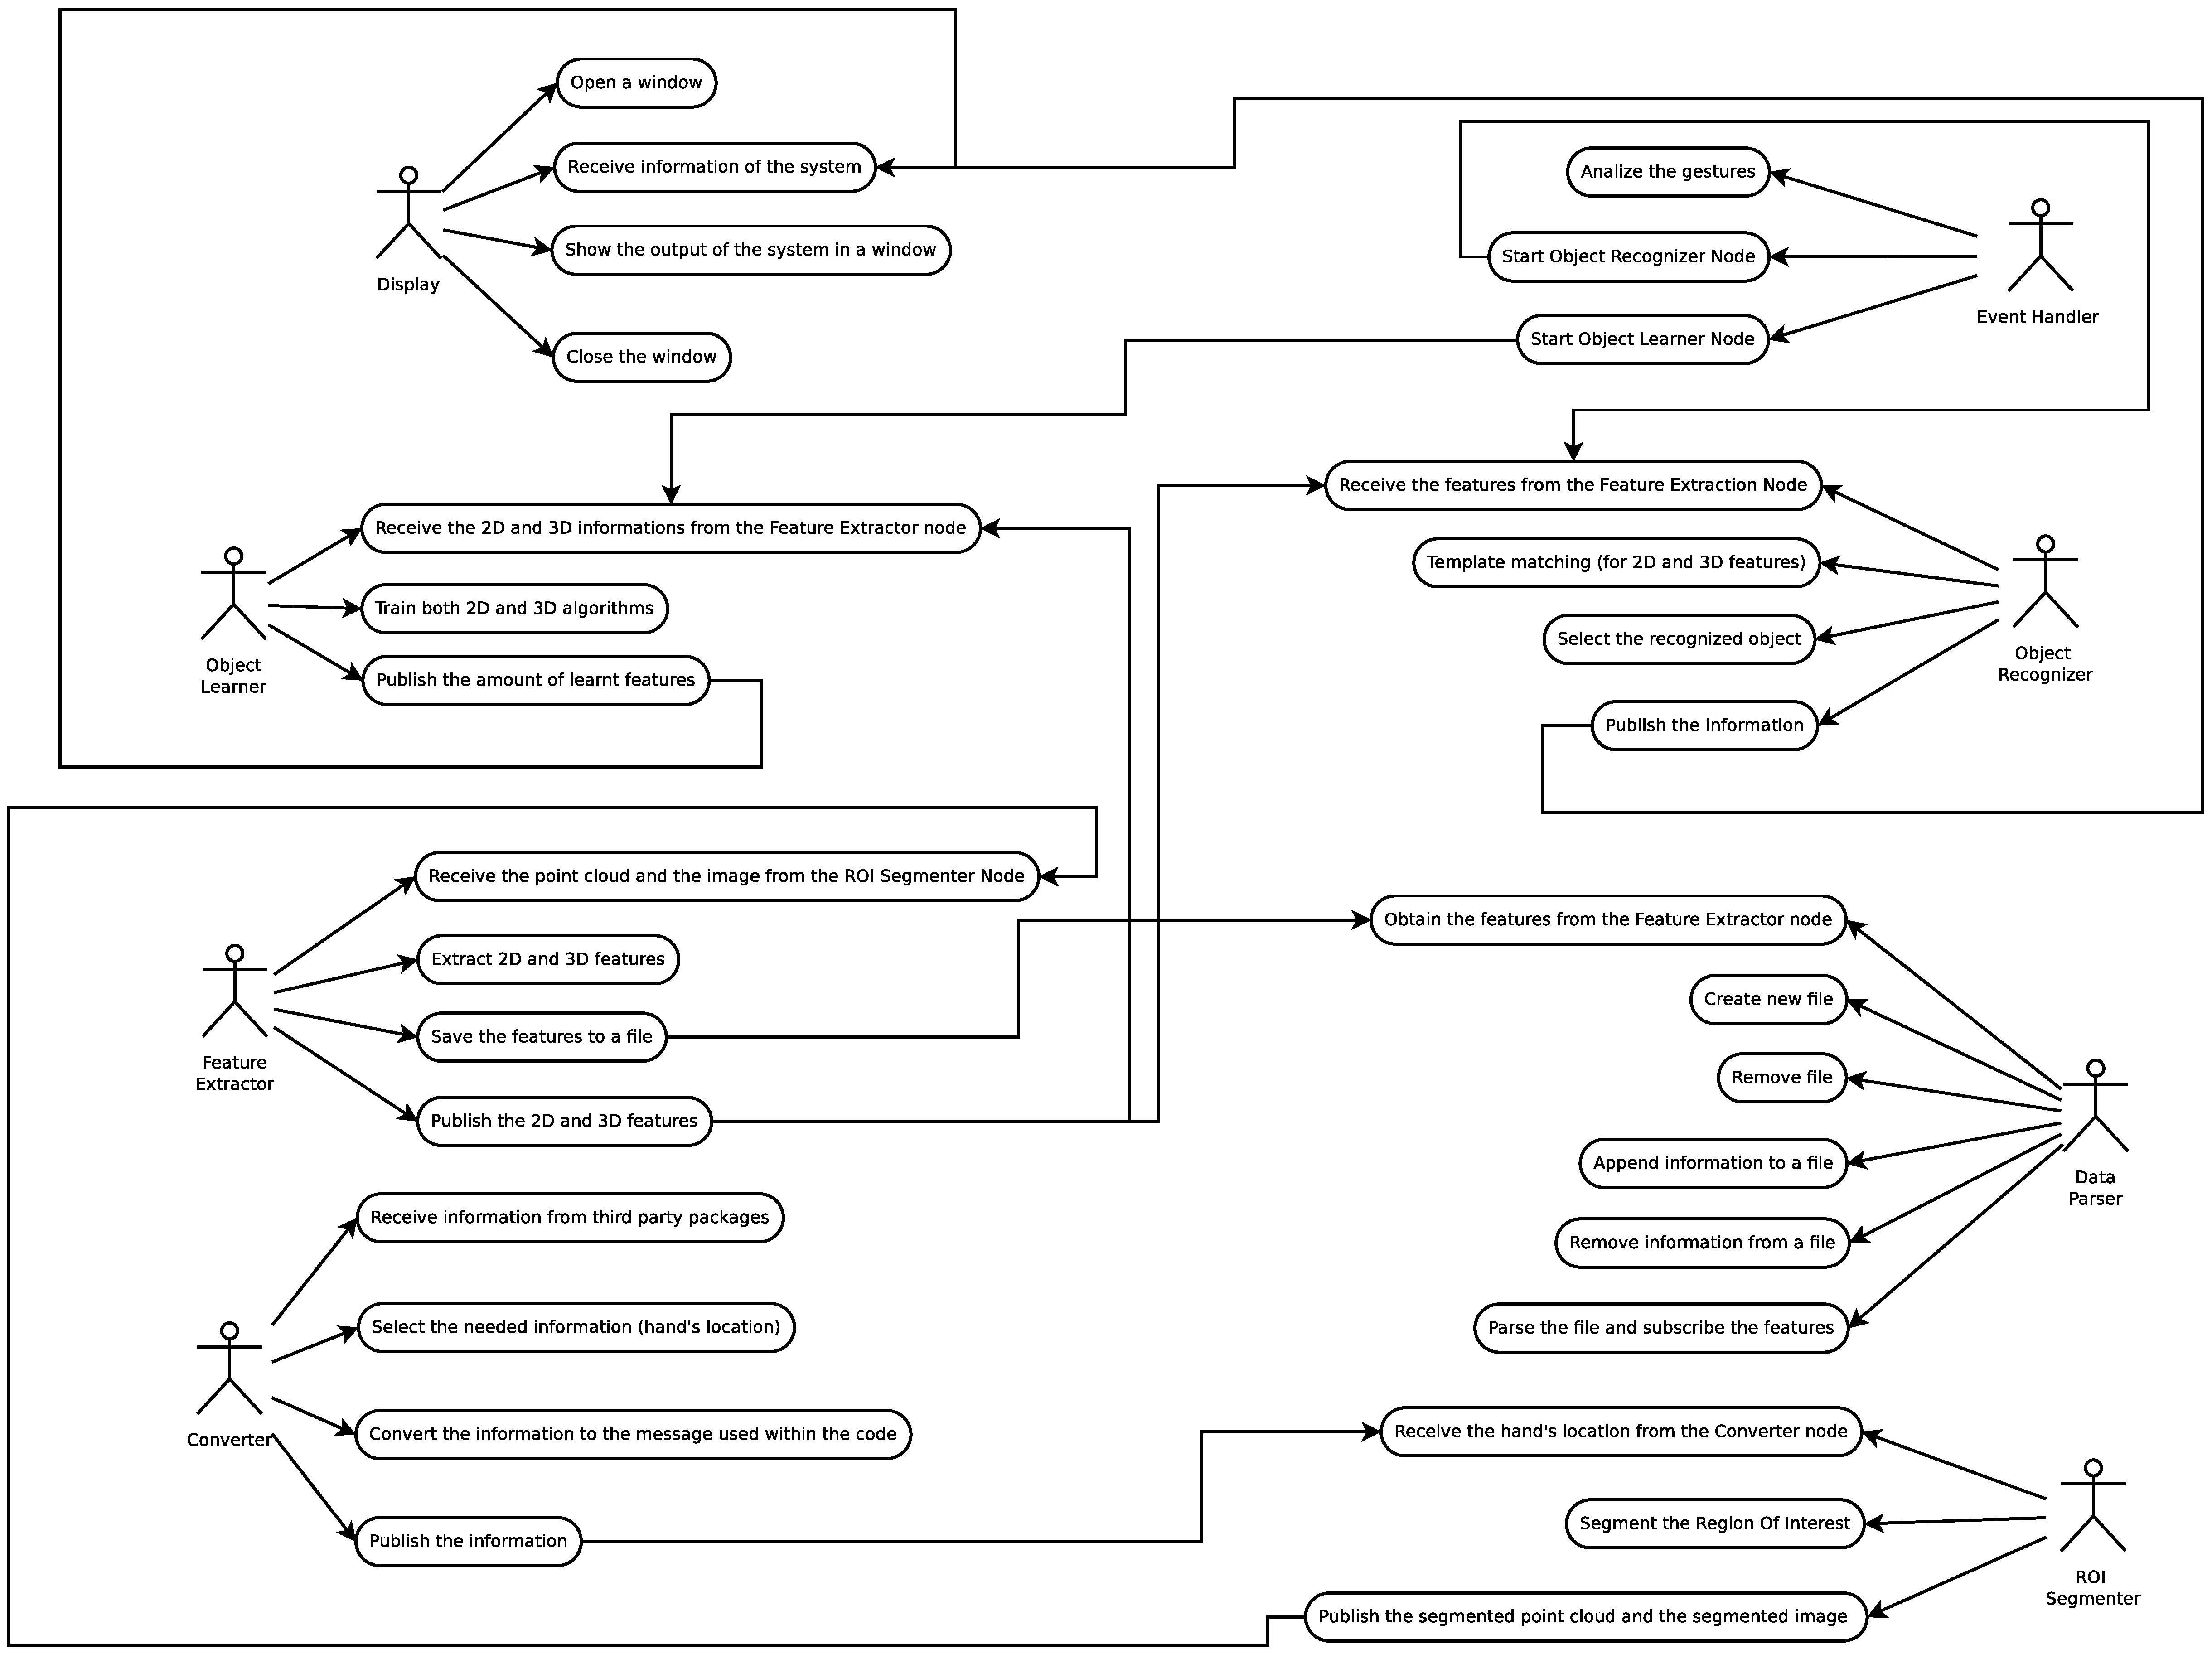
\includegraphics[scale=0.3]{img/diagrams/use_case.eps}
% %\end{center}
% \end{figure}

\subsubsection{Sequence Diagram}
In the following diagram can be seen the interaction between nodes. \\
The Event Handler node triggers the execution of the Recognizer and the Learner nodes. As it was previously mentioned, the triggering event is defined to create a more natural human-machine interaction.
The converter, ROI Segmenters and Feature Extractors nodes are continuously working and publishing the information on their topics. 
Hence, the information needed for the Event Handler, Recognizer and Learner nodes is obtained subscribing to those topics. 
\begin{figure}[H]
\begin{center}
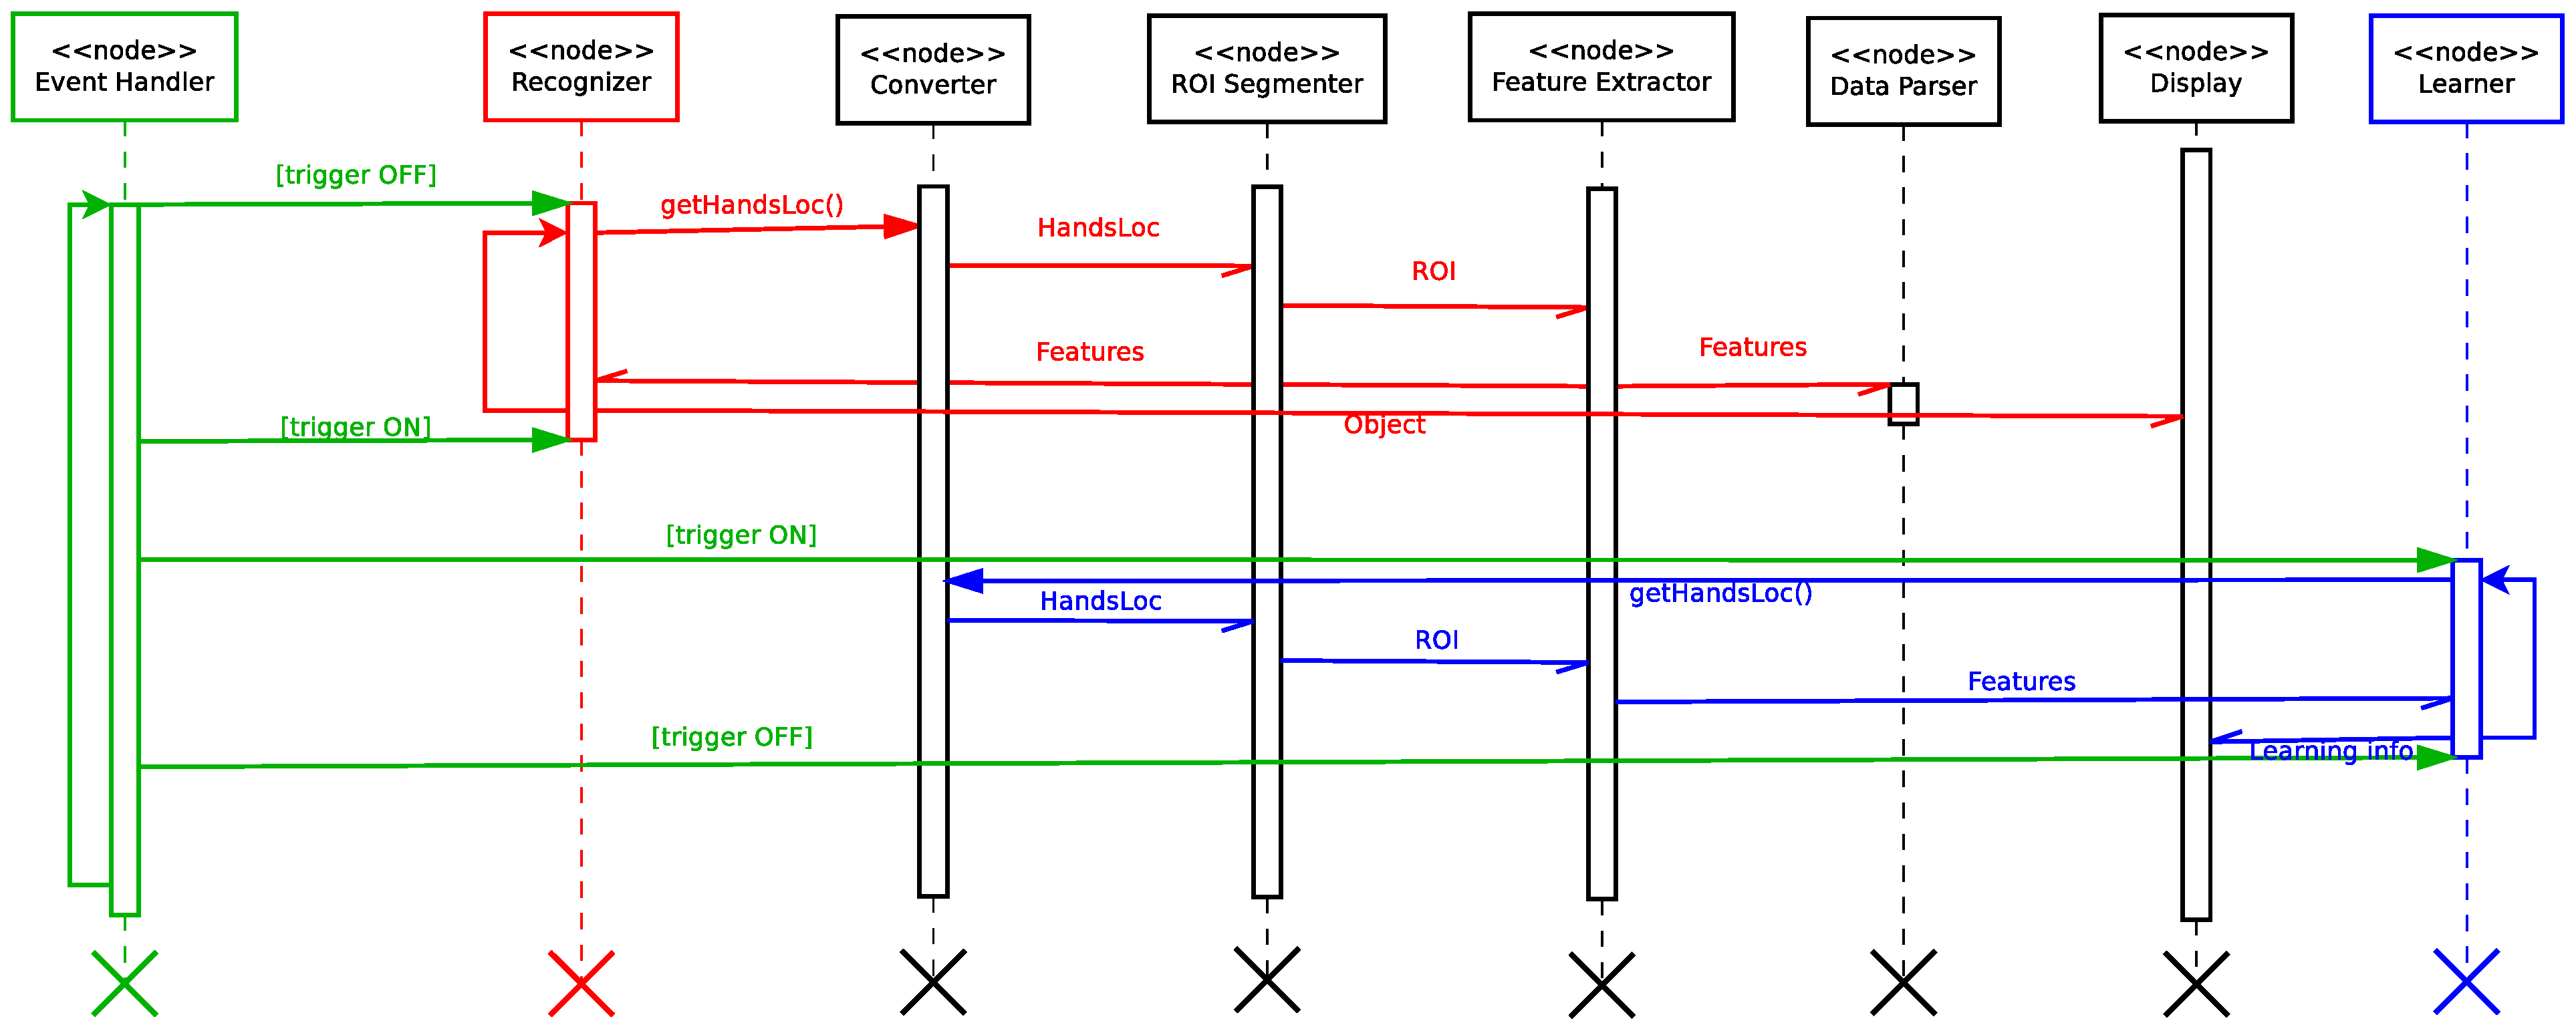
\includegraphics[width=\textwidth]{img/diagrams/sequence.eps}
\end{center}
\end{figure}

\subsection{Flowchart}
In the following diagram, the flow of the program is represented. 
\begin{figure}[H]
\begin{center}
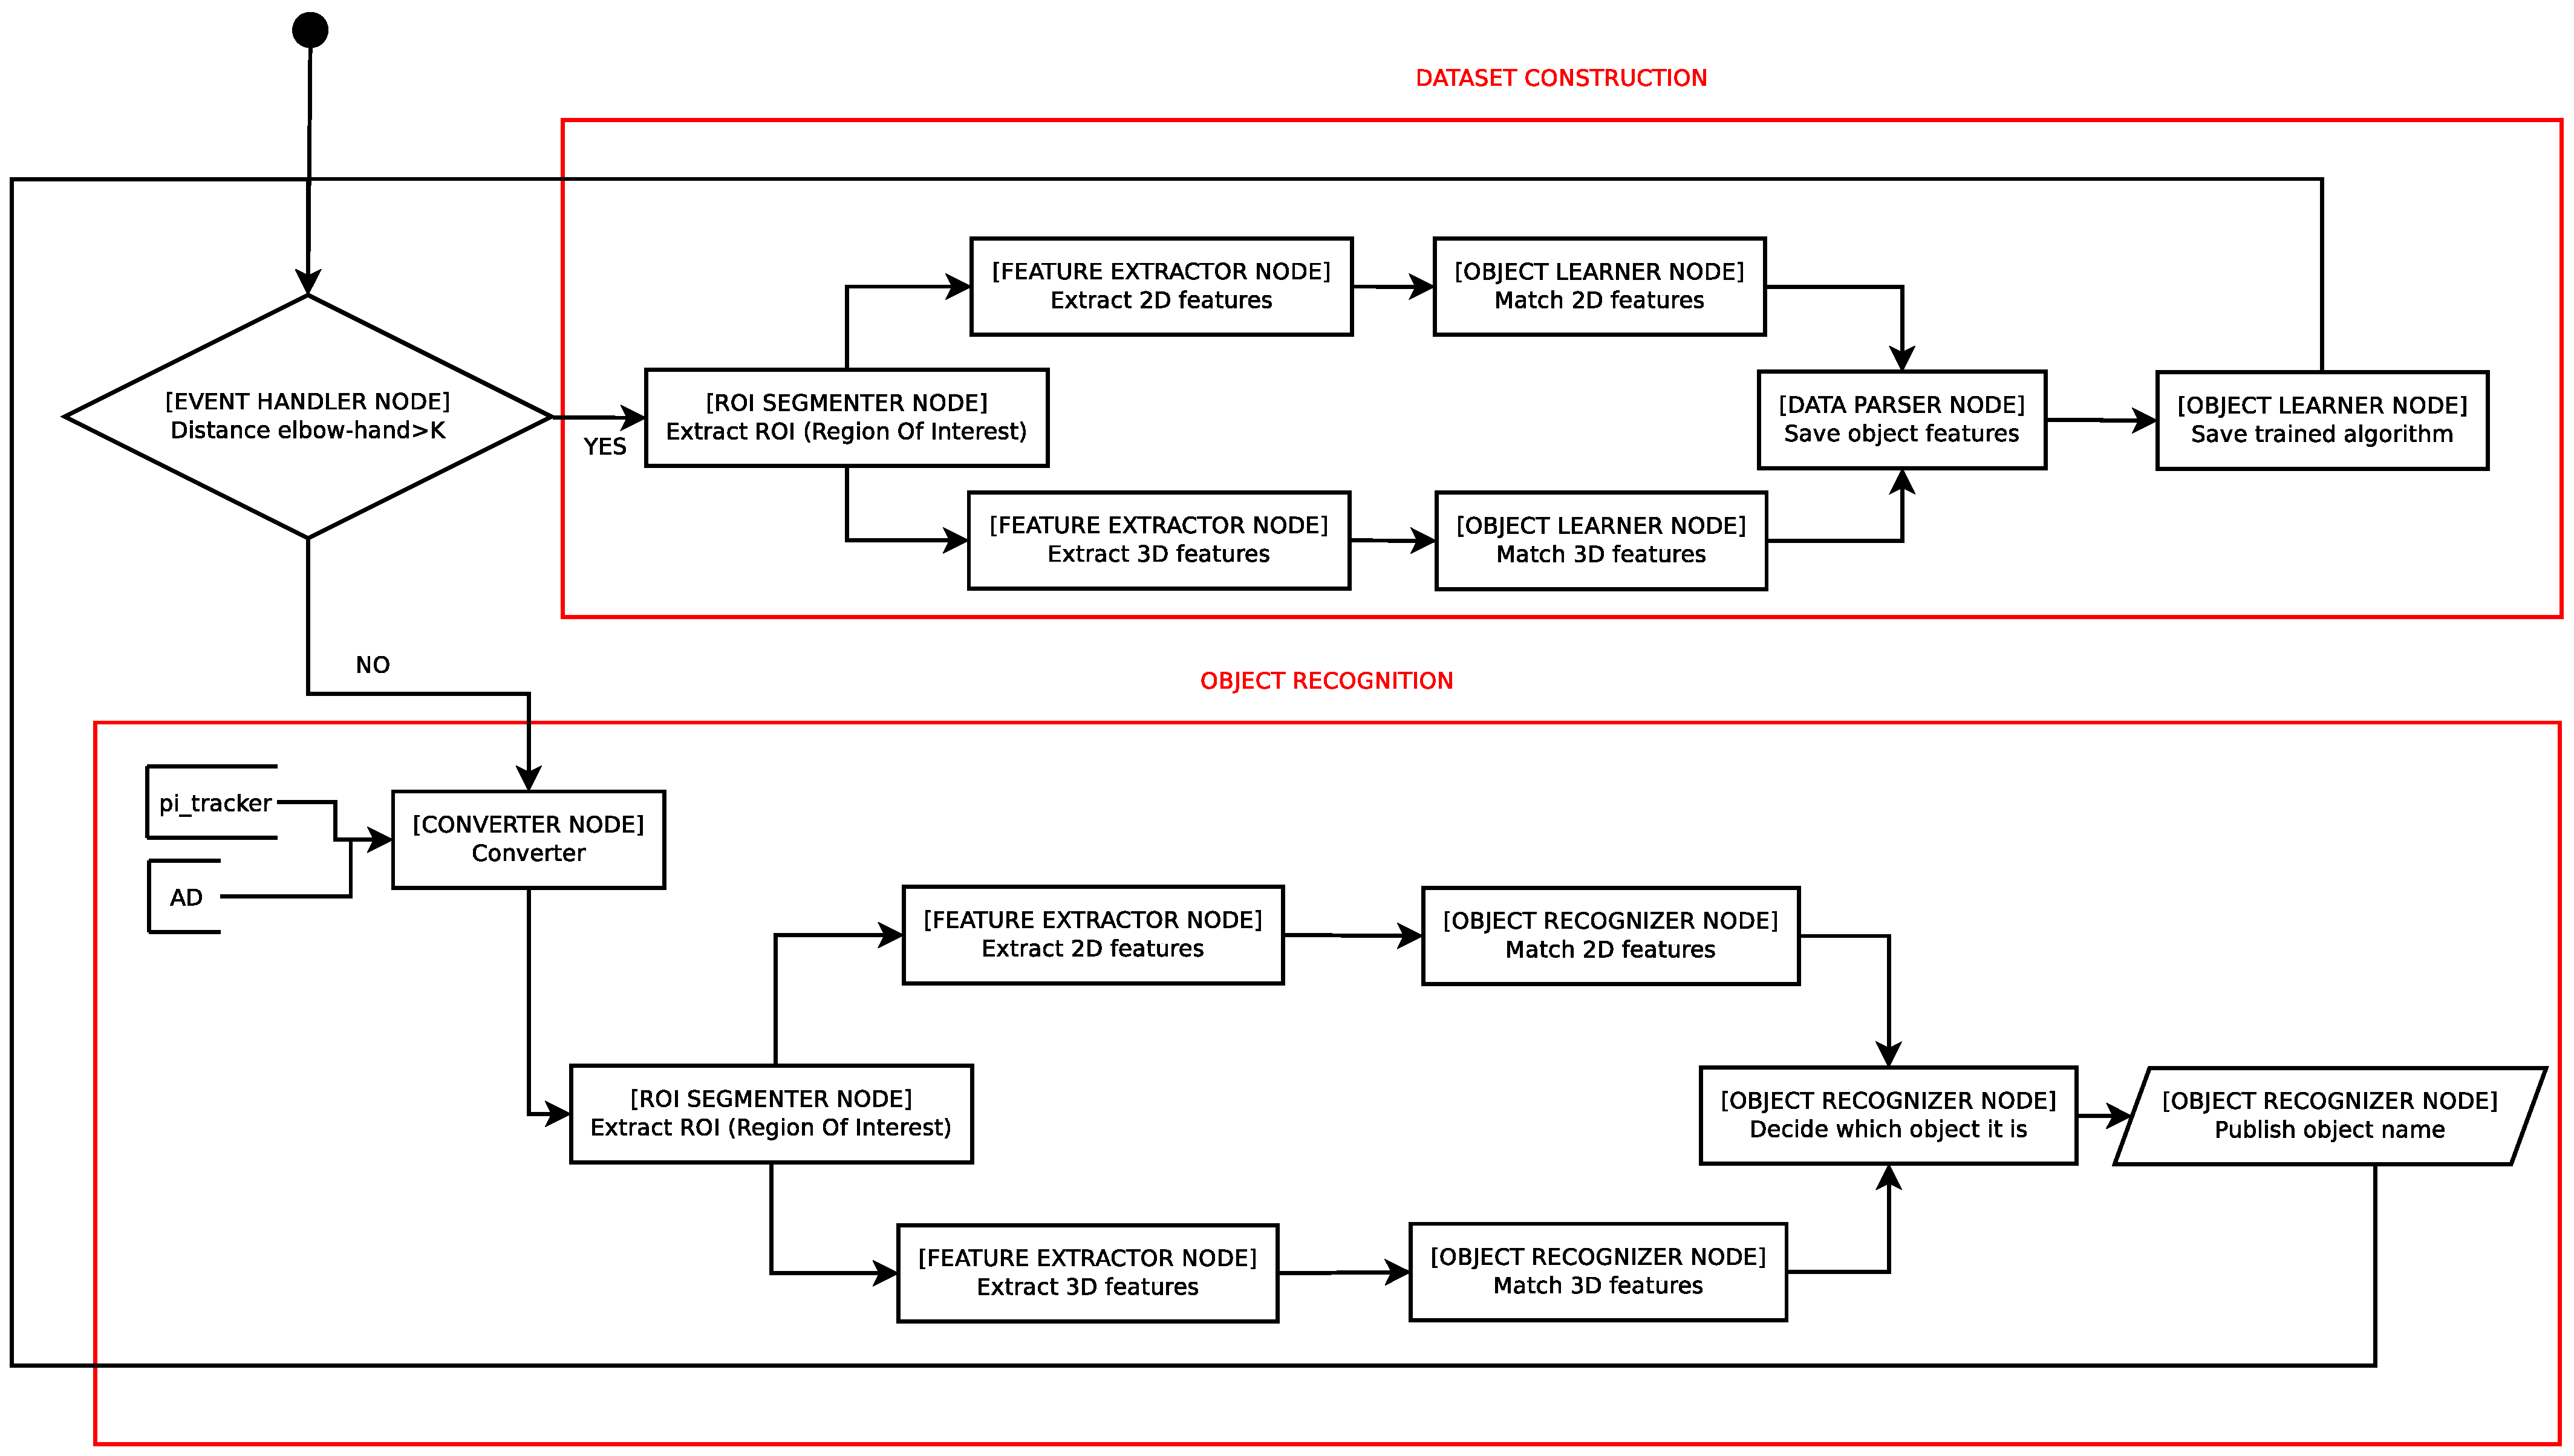
\includegraphics[width=\textwidth]{img/diagrams/flowcharts.eps}
\end{center}
\end{figure}





\section{Functional requirements}

\subsection{General requirements}

\begin{enumerate}[label=\textbf{FR\threedigits*}, leftmargin=2cm]

	\item The software must be developed under ROS (Robotic Operating System), using the Groovy distribution and rosbuild.
	\item A version control system should be used (GIT) and all the code must be periodically updated in the following github repository:  $https://github.com/irenesanznieto/TFG$
%	\item The software has to have an interface. Its requirements are specified in the following "Interface Requirements" section. 
	\item The software must accept as inputs the following RGB-D sensors: Microsoft Kinect, ASUS Xtion PRO, ASUS Xtion PRO Live, PrimeSense PSDK 5.0.
	\item The output of the system must be a topic specifying the name of the detected object. 
 
 
\hspace*{-2cm}\subsection{Converter}

\item The information must be received subscribing to the topics of the different third-party packages. 
\item This node must convert different message formats to the custom message used within this project, serving as an interface. 
%\item The internal message format must have the following structure: \\[0.3cm]
%\textit{
%std\_ msgs/Header header\\[0.1cm]
%int32 id\\[0.1cm]
%geometry\_ msgs/Vector3[] position\\
%\hspace*{0.5cm}float64 x\\
%\hspace*{0.5cm}float64 y\\
%\hspace*{0.5cm}float64 z\\
%}


\subsection{ROI Segmenters}

   \subsubsection{ROI Segmenter 3D}
	\item This node must segment the Region Of Interest in 3D (point cloud). 
	\item The ROI must be a box around the hand's position. 
	\item The dimensions of the ROI box must be fixed and must have a value suitable for this application.  
   \subsubsection{ROI Segmenter 2D}
   	\item This node must segment the Region Of Interest in 2D (image).
   	\item The original input image must be the one obtained directly from the RGB-D sensor being used.
   	\item The size of the 2D ROI must be extracted from the 3D ROI x and y dimensions. Those measures must be in pixels. 
	\item The 2D ROI must be cropped from the original image using the points obtained from the 3D ROI. 

\subsection{Feature Extractors}
   \subsubsection{Feature Extractor 2D}
	\item This node must extract the 2D features. 
	\item The 2D features will be expressed as a vector of descriptors. %, using the ORB approach. 
	\item The 2D features of all the views of each object will be stored in a file, using the data parser class.  
  
  \subsubsection{Feature Extractor 3D}
   	\item This node must extract the 3D features. 
	\item The 3D features will be expressed as a vector of features. %, using the Line-Mod approach.
	\item The 3D features of all the views of each object will be stored in a file, using the data parser class.  

\subsection{Data Parser}
\item This class compresses the features obtained to have one data file per object with all the information.
 
\item It has to be able to create a new file for storing the features of a new object. 
\item It has to be able to delete certain views or a complete file of the dataset. 
\item It has to be able to add another view to a previously stored object. 

\item This class will also be able to read the files to extract the 2D and 3D features of each object of the dataset. 

\item The name of the file will be the one given to the object. 

% \item The datafile structure will be: \\
% 		\begin{lstlisting}
% 	<view1>
% 		<2D>
% 			[descriptor information ..]
% 		</2D>
% 		<3D>
% 			[template information ..]
% 		</3D>
% 	</view1>	
% 	...
% 	...
% 	...		
			
% 	<viewN>
% 		<2D>
% 			[descriptor information ..]
% 		</2D>
% 		<3D>
% 			[template information ..]
% 		</3D>
% 	</viewN>	
		
% 		\end{lstlisting}
	


 
\subsection{Event Handler}
\item This node must have access to the hand's position information. 
\item This node must launch the object learner node or the object recognizer node depending on a triggering event. 
\item The triggering event occurs when the distance between the hand and the torso is equal or higher than 0.5m.   
 
% \subsection{Display}

% \item The program must have a window with the output of the camera of the kinect sensor. 
% \item The information as to what mode the program is in has to be shown in the title of the window.
% \item In the recognition mode, the interface must show a square around the detected object and a text label indicating the object's name. Also, two points must be drawn in each of the hands. 
% %\item The learning mode should open a new window where an shpere will appear. The sphere must show a different colour when a template of that zone is made. On the main window, a square should be placed around the new object. 
% \item The learning mode should display the number of views obtained and processed of the object as well as an indication as to how to rotate the object to obtain further views. 


\subsection{Object Learner}
	\item The input to this node will be the features (both 2D and 3D) extracted from the feature extractor node. 
	\item This node must have two algorithms, one for 2D and other for 3D. 
%	\item The algorithm used with 2D features should be a BruteForce trainer.
%	\item The algorithm used with 3D features must be the Line-Mod trainer. 	
	% \item This node must send feedback messages to the display with the learning information (number of views of the object processed, information about how to rotate the object).
	\item The output of this node will be the trained algorithms, whose parameters must be written to a file. 

\subsection{Object Recognizer}
	\item This node must have two algorithms, one for 2D and other for 3D. 
%	\item The algorithm used with 2D features should be a BruteForce matcher.
%	\item The algorithm used with 3D features must be the Line-Mod matcher. 
	\item A weighting must be made depending on the amount of texture possessed by each object to decide which matching should have more importance, the 2D or the 3D one. 
	\item A weighting must be made to the previous weighting. This will help reduce the false positives and negatives by modelling occlusions depending on the hand-elbow relative positions. 
	\item The output of this node must be a topic in which the object's name is published.
	






\end{enumerate}



\section{Performance requirements}

\begin{enumerate}[label=\textbf{PR\threedigits*}]
\item The recognition must run on the lowest amount of time possible, to allow a fluid human-robot interaction. This time must be lower than 500 ms. 
\item The learning must run on the lowest amount of time possible, to allow a fluid human-robot interaction. This time must be lower than 5s. 
\end{enumerate}


%\section{Operational requirements}
%\section{Resource requirements}
%\section{Verification requirements}
%\section{Acceptance testing requirements}	%This is a validation activity; did we build the right thing? Is this what the customer really needs? 

\section{Documentation requirements}
\begin{enumerate}[label=\textbf{DR\threedigits*}]
	\item The code must be completely documented, i.e. each class, class function , class member and piece of code should have comments explaining all the aspects. 
	\item The documentation will be made using Doxygen notation, through the rosdoc\_ lite 
	% $[http://wiki.ros.org/rosdoc\_lite]$ 
	ROS package. 
	\item All the documentation must be available at the git repository. 
\end{enumerate}

%\section{Security requirements}
%\section{Portability requirements}
%\section{Quality requirements}
%\section{Reliability requirements}
\section{Maintainability requirements}
\begin{enumerate}[label=\textbf{MR\threedigits*}]
	\item The code must be as modular as possible. 
	\item All the classes' variables that are susceptible of being modified through a inheritance will be declared as protected. 
	\item Gtests will be built to demonstrate each functional requirement. 
	
\end{enumerate}

%\section{Safety requirements}

%\section{Time Schedule}


\end{document}
